\chapter{Implementation}
\label{Implementation}
This chapter describes the implementation details of the system and shows the internal architecture. All system components are implemented in Typescript that is later compiled to JavaScript. This choice of language enables code sharing between individual components and allow us to support multiple platforms (desktop via Node.js, and browser). All system components are dependent on Explorer-core module where is the whole database system implemented (see Figure \ref{systemArchitecture}). 


\begin{figure}[h]
    \centering
    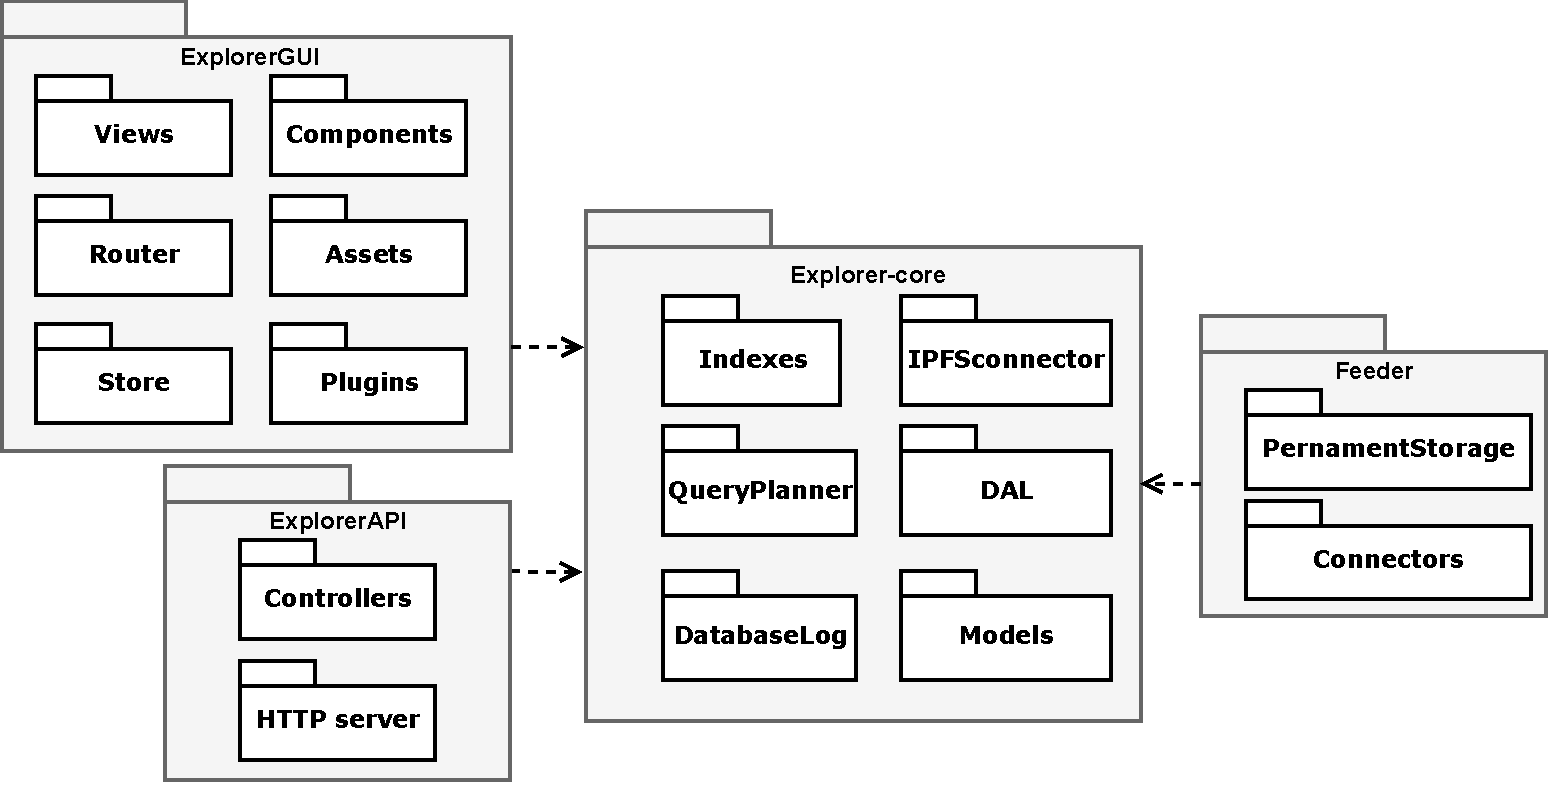
\includegraphics[width=\textwidth]{ExplorerArchitecture.pdf}
    \caption{System architecture}
    \label{systemArchitecture}
\end{figure}


\section{Explorer-core Implementation}
Explorer-core is the most complex module of a whole system with more than 5,000 lines of code. The database subsystem is a main part of the Explorer-core module. The subsystem consists of a query system, indexes and an abstract database layer. Explorer-core is only system components that communicates with IPFS via js-ipfs\footnote{\url{https://github.com/ipfs/js-ipfs}} implementation.

\subsection{IPFS Connector}
IPFS connector is a singleton class that provides a connection to IPFS. It has a method \texttt{getInstanceAsync} which will return promise that resolves into IPFS node instance. This instance is stored in a private static class variable. Next call of function \texttt{getInstanceAsync} returns that static class variable.
Also, swarm key is present in IPFS connector. This key is used to make private IPFS network with only Explorers and Feeders. Other peers (without swarm key) can not connect to our network. IPFS connector contains settings for node.js and browser IPFS peer. Browser peers use WebRTC and WebSockets for transport. Node.js peers use TCP and WebSockets. That means that Feeders (a node.js application) can communicate with each other with TCP. Explorer communicates with other explorers with WebSockets or WebRTC. Explorer uses WebSockets when communicating with Feeders.

\subsection{Indexes}
For indexing purposes, there is currently implemented only B-tree, but different structures such as tries\footnote{\url{https://en.wikipedia.org/wiki/Trie}} can be employed easily. They only need to implement index interface (function such as \texttt{insert}, \texttt{delete}, \texttt{update}, \texttt{find}). We can create indexes on database entities with decorators\footnote{\url{https://www.typescriptlang.org/docs/handbook/decorators.html}}, which are part of ECMAScript 6 standard. Every database entity has to have \texttt{PrimaryKey} decorator on property that is used as a primary index. Index has three parameters:
\begin{itemize}
    \item \texttt{comparator} -- is a function that accepts two arguments and returns number that is less than zero if the first argument is greater than a second, zero if arguments are the same, more than zero if a second argument is greater than first. If a user has not set any custom comparator default one (\texttt{(a, b) =>
    a < b ? -1 : +(a > b)}) is used. This default comparator works on atomic keys such as string or numbers. 
    \item \texttt{keyGetter} -- is another function that accepts a whole entity as arguments and returns key, that is used in an index. A~default key getter is function that returns value of index property (for example default key getter for property \texttt{height} is \texttt{(e) =>  e[''height'']}).
    \item \texttt{branching} -- the branching factor is the number of children at each node (the outdegree). Default branching factor is 16.
\end{itemize}

The B-tree structure (see Figure \ref{btree}) is optimized for IPFS. Unlike PostgreSQL B-tree\footnote{\url{https://github.com/postgres/postgres/tree/master/src/backend/access/nbtree}}, leaf nodes have not got left and right sibling references due to cyclic reference that is not possible in IPFS, because links are changing CID of an object \cite{stonebraker1986design}. Therefore, if we store object \texttt{A} with a link to the object \texttt{B}, CID of \texttt{A} will change. Then if we add backlink from \texttt{B} to \texttt{A}, CID of \texttt{B} will be changed and so \texttt{A} is now linked to an old version of \texttt{B}. If we update link of object \texttt{A} to point on the new version of object \texttt{B}, CID of object \texttt{A} will change and therefore object \texttt{B} is now pointing to the old version of object \texttt{A}. From this example, it appears that there is no way of making cyclic references in IPFS. Without siblings's references, we do not have to store data only in leaves, but we can store data in nodes itself. This approach leads to better performance when executing queries. For insert queries, statistically fewer nodes need to be updated. Also in search queries, there is a chance that we would found a key in some non-leaf node; therefore, we would need fewer node visits.

All search queries (equal, less, greater, between) has two steps:
\begin{itemize}
    \item \textbf{Find subtree} -- First, we need to find minimal subtree that contains all results. We start in a root node of the B-tree. Then, we use an index \texttt{comparator} function to determine if we can visit some child node and still have all the result in it. If not, then we have found a minimal subtree for the query.
    \item \textbf{Traverse} -- To get results of the query, we can traverse minimal subtree in two directions. In-order for \texttt{greater than} and \texttt{between}. For \texttt{less than} reversed in-order. With \texttt{equal}, it does not matter.
\end{itemize}

\begin{figure}[h]
    \centering
    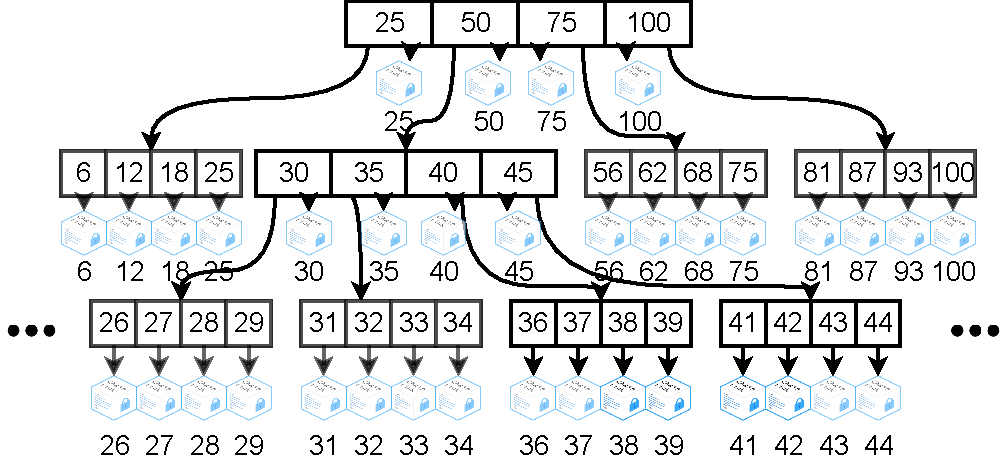
\includegraphics[width=\textwidth]{btreeindex.pdf}
    \caption{B-tree indexing first 100 blocks by their height}
    \label{btree}
\end{figure}

\subsection{Query System}
Our database offers a complex query system. A~query can consist of multiple conditions, and the \texttt{Query Planner} is responsible for resolving them. It decides which indexes are used for query and choose a strategy. If there is no condition, a primary key is used for query execution. In the case of a single condition, \texttt{Query Planner} checks if there is an index on the condition's property. If yes, then this index is used to perform the query. Else condition is transformed to filter, and a primary key is used to obtain results which are then filtered. For multiple conditions connected with logical operators \texttt{AND} or \texttt{OR}, \texttt{Query Planner} creates \texttt{OR-hashset} and \texttt{AND-hashset}. \texttt{AND-hashset} is initialized with the results of a condition which has the smallest number of results and uses \texttt{AND} operator. Then we check for each result hash for all other \texttt{AND} conditions if \texttt{AND-hashset} contains it. If no, a hash is deleted from \texttt{AND-hashset}. This creates intersection between all \texttt{AND} conditions. The \texttt{OR-hashset} is created empty. Then, we add a hash of every result of all \texttt{OR} conditions to it. This creates union between \texttt{OR} conditions. At the end, we perform union between \texttt{AND-hashset} and \texttt{OR-hashset}. This creates final hashset which is used later to obtain actual data with resolvers such as \texttt{all}, \texttt{first}, \texttt{paginate} etc. If one of the \texttt{AND} conditions has great selectivity (it has less than a hundred results), \texttt{Query Planner} can decide to don't use other indexes, but transform condition to filter and cycle over the results. Example query returning blocks between 38 and 42 is shown in Figure \ref{btreeQuery}. A~peer needs to download only data that are highlighted in green. After downloading them, they are stored on a peer's filesystem and are offered to other peers. 

\begin{figure}[h]
    \centering
    \includegraphics[width=\textwidth]{btreeIndexQuery.pdf}
    \caption{Data access for performing query that returns blocks that have a height between 38 and 42.}
    \label{btreeQuery}
\end{figure}


We can make queries with every database table model (such as model on Figure \ref{classExample}). Whole query system is displayed in the state diagram on the Figure \ref{queryStateDiagram}. The query system consists of these functions: 
\begin{itemize}
    \item \texttt{where(propertyName)} -- create a condition on the property. There can be multiple conditions in one query. A~condition hash needs to be followed by one of the functions: 
    \begin{itemize}
        \item \texttt{gt(value)} -- property is greater or equal than \texttt{value}. The \texttt{Query Planner} finds in an index first object that has property (set by \texttt{propertyName} in \texttt{where} function) equal or greater than \texttt{value}, and traverse index to the right (to bigger objects);
        \item \texttt{lt(value)} -- property is less or equal than \texttt{value}. Similar as in the \texttt{gt} function, the QueryPlanner finds the closest object that has property equal or less than \texttt{value}. Then, the query traverses index to the smaller objects with smaller index value (to the left);
        \item \texttt{between(min, max)} -- property is greater or equal than \texttt{min} and less or equal than \texttt{max};
        \item \texttt{equal(value)} -- returns all objects that \texttt{keyGetter} function returns same key as \texttt{value};
    \end{itemize}
    \item \texttt{skip(offsetValue)} -- query will skip \texttt{offsetValue} number of results;
    \item \texttt{limit(limitValue)} -- set maximum number of results. After query has \texttt{limitValue} count of matched objects it will stop browsing the index;
    \item \texttt{all()} -- return all objects that matched query;
    \item \texttt{first()} -- return the first object that matched a query;
    \item \texttt{and(childQuery)} -- logical and between two queries. Parent query resolves \texttt{childQuery} (call \texttt{all()} function) and add its results to \texttt{AND-hashset};
    \item \texttt{and(property)} -- Thanks to available generic programming\footnote{\url{https://en.wikipedia.org/wiki/Generic_programming}} in Typescript, \texttt{and} can be also called with string argument. This register another query condition;
    \item \texttt{or(childQuery)} -- logical or between two queries; \texttt{childQuery} will be resolved when parent query needs it, and its results stored in \texttt{OR-hashset} of parent query;
    \item \texttt{or(property)} -- similar as \texttt{and} function, \texttt{or} can be also called with string parameter. This register another condition to query;
    \item \texttt{iterate()} -- returns iterator that can be used in \texttt{for (result of query)} cycle.
\end{itemize}


\begin{figure}[h]
    \centering
    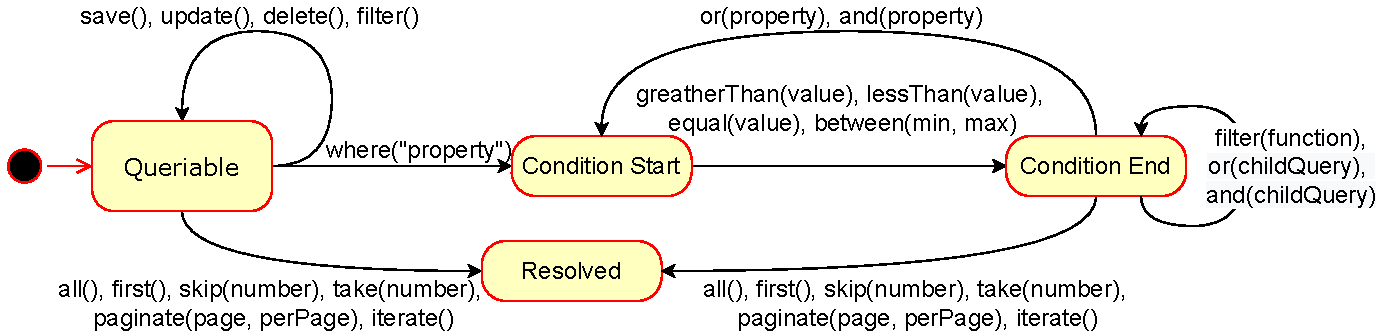
\includegraphics[width=\textwidth]{queryStateDiagram.pdf}
    \caption{State diagram of the query system}
    \label{queryStateDiagram}
\end{figure}


\subsection{Database}
The most important part of the Explorer-core module is the database subsystem which connects the query system with indexes. When we make a query, it is precessed by database, and data are obtained with the help of the indexes.

\subsubsection{Tables}
A~database contains tables that consist of indexes. A~table has an interface that provides operations to modify table data:
\begin{itemize}
    \item \texttt{create} -- creates history log for entity with first entity version. Then adds it to every table index;
    \item \texttt{update} -- adds new version of the entity to its history log. Then update every index of the table;
    \item \texttt{delete} -- removes entity from every table index. From now, an entity can not be found in this table.
\end{itemize}
There is no \texttt{select} operation because a table itself does not perform queries for obtaining data (table has not got necessary logic for choosing optimal index for query). Selects are performed by \textit{Query Planner} after analysing all query conditions.

Example of the class User is in Figure \ref{classExample}. It has two indexes. One primary on property \texttt{name} and one normal index on property \texttt{age}. The second index has also specified \texttt{comparator} that is a bit faster than default one but works only on numbers, and \texttt{keyGetter} that returns a year when a user has born. 

\begin{figure}[h]
    \centering
    \begin{lstlisting}[style=ES6]
    class User extends Queriable<User> {
        @PrimaryKey()
        name: string;

        @Index(
            (a, b) => a - b,
            u~=> new Date().getFullYear() - u.age,
        )
        age: number;
    }
    \end{lstlisting}
    \caption{Example of database table abstraction }
    \label{classExample}
\end{figure}



\subsubsection{Transactions}
A~database can execute only a single transaction at the time to prevent data inconsistency. For that reason, we implemented a transaction queue where transactions are stored before executing in the order in which they came. Executing more transactions in a row is significantly more effective than executing them one by one. If a transactions queue has only one transaction, it waits 50 ms for more transactions to come. Transactions in our system are represented by classes \texttt{Transaction} and \texttt{TransactionsBulk}. Both classes implements \texttt{ITrasnaction} interface with \texttt{run} function. Transactions bulk are treated the same way as a single transaction thanks to Composite pattern\footnote{\url{https://en.wikipedia.org/wiki/Composite_pattern}} (see Figure \ref{transactionsComposite}). After executing, each transaction is appended to the database log. After we execute all transactions in transactions queue (transaction queue is empty), we publish a new database version to all connected peers.

\begin{figure}[h]
    \centering
    \begin{lstlisting}[style=ES6]
        interface ITransaction{
            run();
        }
        
        public class Transaction implements ITransaction {
            operation: DbOperation;
            data: any;
            run() {
                ...
            }
        }
        
        public class TransactionsBulk implements ITransaction {
            public transactions: ITransaction[];
            public run() {
                for (const transaction of this.transactions)
                    await transaction.run(database);
            }
        }
    \end{lstlisting}
    \caption{Transactions use composite pattern. Body of function \texttt{run} of the \texttt{Transaction} class is omitted due to complexity.}
    \label{transactionsComposite}
\end{figure}


\subsubsection{Synchronization}
There are two types of transactions: 1) those that changes the database state (\texttt{create}, \texttt{update}, \texttt{delete}); and 2) those that do not (\texttt{select}). Every transaction that changes the database state needs to be synchronized with other peers. We created Database log for that. It is an append-only log with a discrete-time. Every entry of a database log has these properties:
\begin{itemize}
    \item \textbf{hash} -- an IPFS hash of this entry;
    \item \textbf{payload} -- payload is object that contains all entry data. Usually, there is a transaction (or transactions bulk if more transactions are published in this entry) and an IPFS hash of the database;
    \item \textbf{parent} -- an IPFS hash to previous entry. We can re-create a whole database log from a head entry be accessing parent property until it is \texttt{null};
    \item \textbf{clock} -- A~Lamport clock \footnote{\url{https://en.wikipedia.org/wiki/Lamport_timestamps}} with entry create time.
\end{itemize}
There can be only one valid database transaction at every point in time. There are several strategies to choose which transaction is globally accepted and which transactions need to rollbacks (described in design \ref{designSync}). Merging database logs is a common operation in our database system. Every time a peer publishes new database version, other peers need to merge this version with theirs.

Example of merging database logs can be seen in Figure \ref{syncDB}. In this example there are two peers (\texttt{Node A} and \texttt{Node B}). First three database version (\texttt{A1}, \texttt{B1}, \texttt{A2}) follows each other and there is no problem with them. But versions \texttt{A3} and \texttt{B2} are published in the same time. Node A~and B do not know about this issue yet, so they both publish another version (\texttt{A4} and \texttt{B3}) on top of their head. After nodes get notified about each other versions, their logs are merged by database log class function \texttt{merge} which accepts another log as a parameter (see Figure \ref{dblogMergeAlgo}). 

At first, we create a new instance of \texttt{TransactionsBulk} where we store transactions that we may need to rollback. Then we check if both logs heads are published at the same time. If one head clock time is greater than another head clock time, we need to get previous database log entry from this log with the same time as another log head to be able to compare these versions. Luckily, both logs head from our example (\texttt{A4}, \texttt{B3}) are published at the same time. We can get a previous entry from accessing \texttt{parent} property of database log entry. Finally, after we got both logs heads from the same time, we can start traversing them and comparing their parents. If logs have the same parent (in our example it is version \texttt{A2}), we found a database version where the fork began. Now, peers need to decide which version of the database to accept. The simplest method is to compare hashes of database log entries. In our example \texttt{A3} entry has bigger hash than \texttt{B2}. This means that \texttt{Node B} needs to rollback transactions published in versions \texttt{B2} and \texttt{B3} and apply them after \texttt{A4}. After the merge, database log has a single head again and all published transactions have been applied.

\begin{figure}[h]
    \centering
    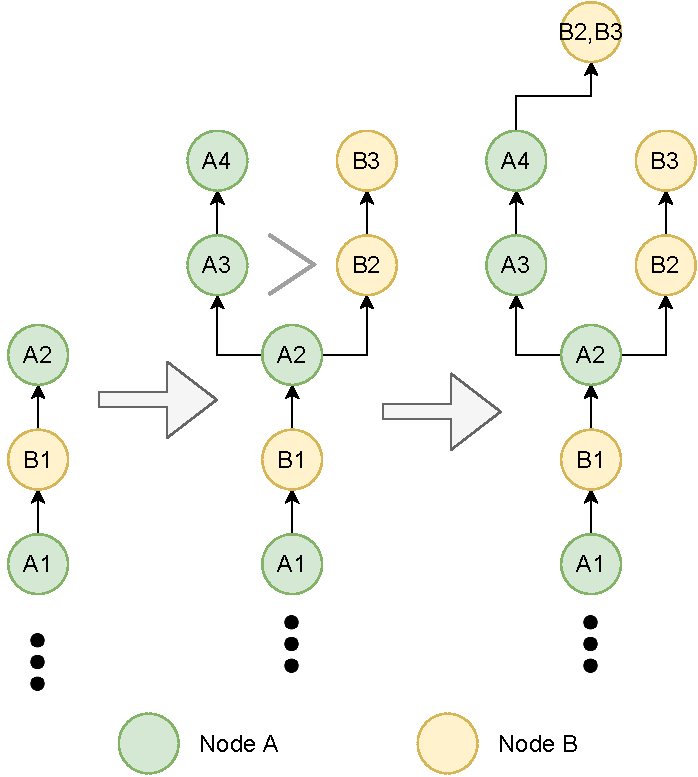
\includegraphics[width=10cm]{syncDB.pdf}
    \caption{Database synchronization}
    \label{syncDB}
\end{figure}

\begin{figure}[h]
    \centering
    \begin{lstlisting}[style=ES6]
public async merge(log) {
    let thisHead = this.head;
    let otherHead = log.head;
    const rollbackOperations = new TransactionsBulk();
    while (thisHead.clock.time != otherHead.clock.time) {
        if (thisHead.clock.time > otherHead.clock.time) {
            if (thisHead.identity.isMe())
                rollbackOperations.push(thisHead.transaction);
            thisHead = await this.get(thisHead.parent);
        } else {
            otherHead = await log.get(otherHead.parent);
        }
    }
    while (thisHead.payload.parent != otherHead.parent) {
        if (thisHead.identity.isMe())
            rollbackOperations.push(thisHead.payload.transaction);
        otherHead = await log.get(otherHead.parent);
        thisHead = await this.get(thisHead.parent);
    }
    if (otherHead.compare(thisHead.hash)) {
        await this.migrate(log, rollbackOperations);
    }
}
    \end{lstlisting}
    \caption{Simplified code for merging database logs}
    \label{dblogMergeAlgo}
\end{figure}

\section{Feeder}
A~Feeder is a simple command-line application written in Typescript. Feeder high-level operation is described in Algorithm \ref{feederAlgo}. It strongly depends on the Explorer-core module. Currently, we support only Blockbook connector as a source of blockchain's data. However, Feeder can be simply expanded to support more data source such as InsightAPI or direct connection to a blockchain as a full node. Each Feeder has configuration file (usually called \texttt{.env}) with Feeder's settings. Main Feeder settings are \texttt{URL} of the source for the blockchain's data and \texttt{DB\_NAME} which is a name of the database where Feeder inserts new blocks. A~Feeder can be connected to only one blockchain. We can create multiple Feeders for single blockchain, but we need to provide some deterministic algorithm, that ensures that each block is parsed by only one Feeder. This can be done by providing \texttt{FeederId} and \texttt{FeedersCount}  in \texttt{.env} config file. If those values are provided, Feeder parses only blocks that have height modulo \texttt{FeedersCount} equals to \texttt{FeederId}. 


\begin{algorithm}[H]
    \SetAlgoLined
    load configuration\;
     \While{there is new block}{
         fetch block\;
         \For{transaction in block}{
            save transaction\;
            }
          save block\;
     }
    \caption{Simplified Feeder algorithm}
    \label{feederAlgo}
\end{algorithm}


\subsection{ExplorerGUI}
ExplorerGUI is a single page application with a simple user interface implemented with Vue.js\footnote{\url{https://vuejs.org/}} that runs in a browser. We use Vuetify\footnote{\url{https://vuetifyjs.com/}} as a user interface library and browser implementation of IndexedDB\footnote{\url{https://developer.mozilla.org/en-US/docs/Web/API/IndexedDB_API}} as a storage for IPFS. Communication with other peers is provided though WebRTC\footnote{\url{https://webrtc.org/}} and WebSockets because a web page in a browser can not open TCP socket. Every opened ExplorerGUI browser tab is the same IPFS node instance. Opening a new tab in incognito mode or different browser spawns new IPFS node.


\begin{figure}[h]
    \centering
    \begin{subfigure}[t]{.5\textwidth}
        \centering
        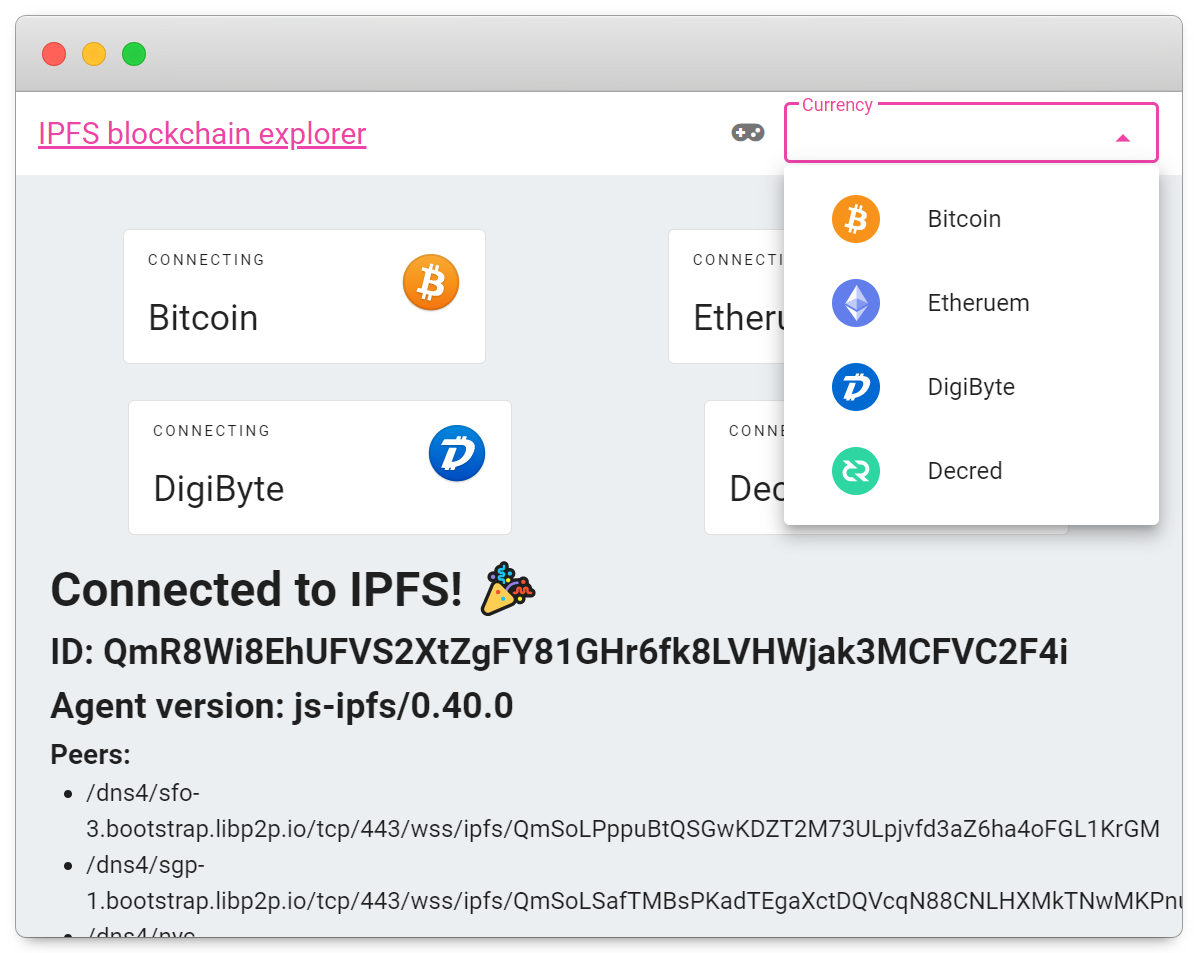
\includegraphics[width=1.0\linewidth]{explorerGuiHomeFrame.png}
        \caption{Home view}
        \label{homeView}
    \end{subfigure}%
    \begin{subfigure}[t]{.5\textwidth}
        \centering
        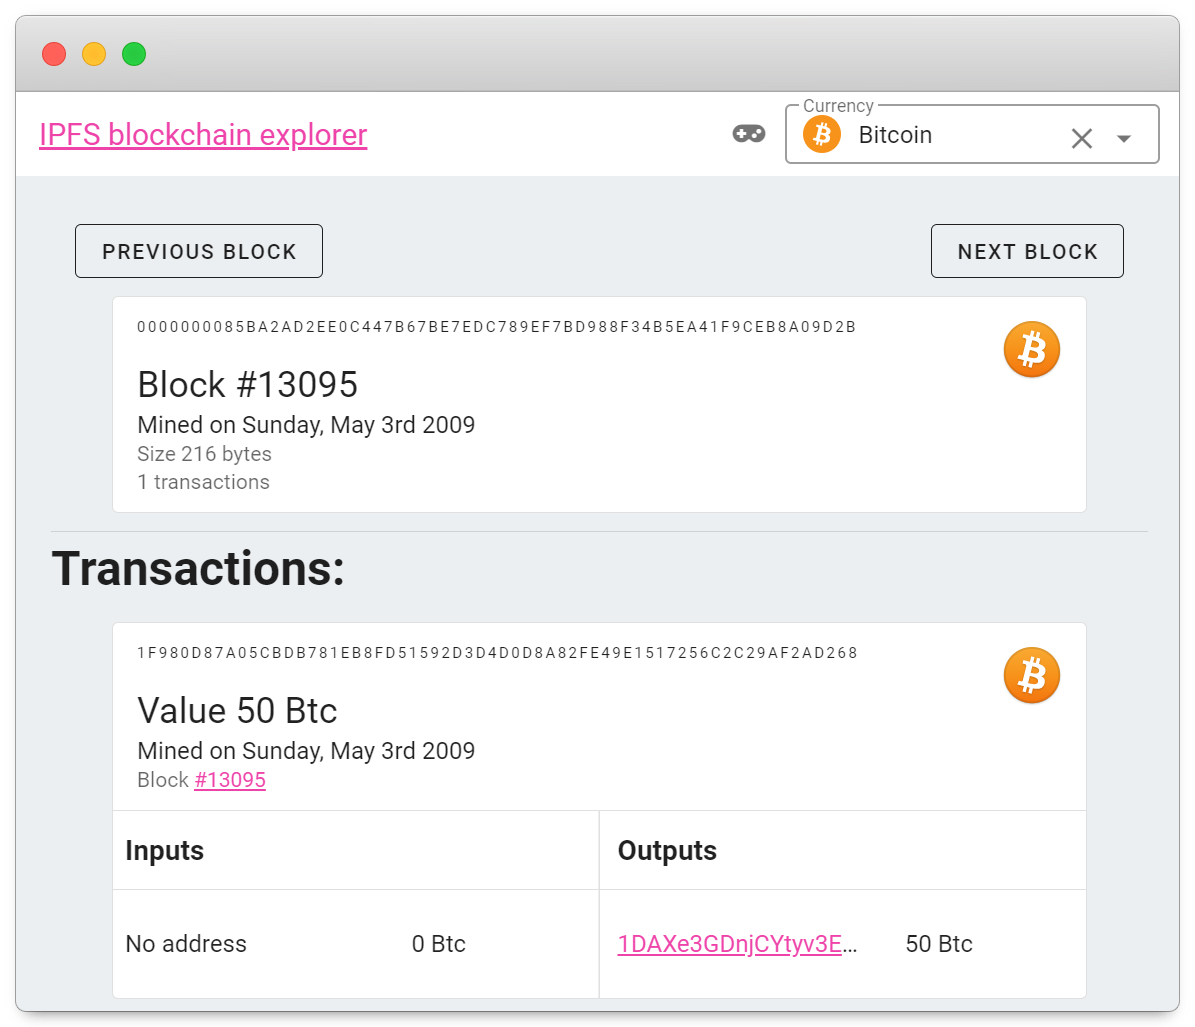
\includegraphics[width=1.0\linewidth]{explorerGuiBlockDetailFrame.png}
        \caption{Block detail view}
        \label{blockDetailView}
    \end{subfigure}
    \begin{subfigure}[t]{.5\textwidth}
        \centering
        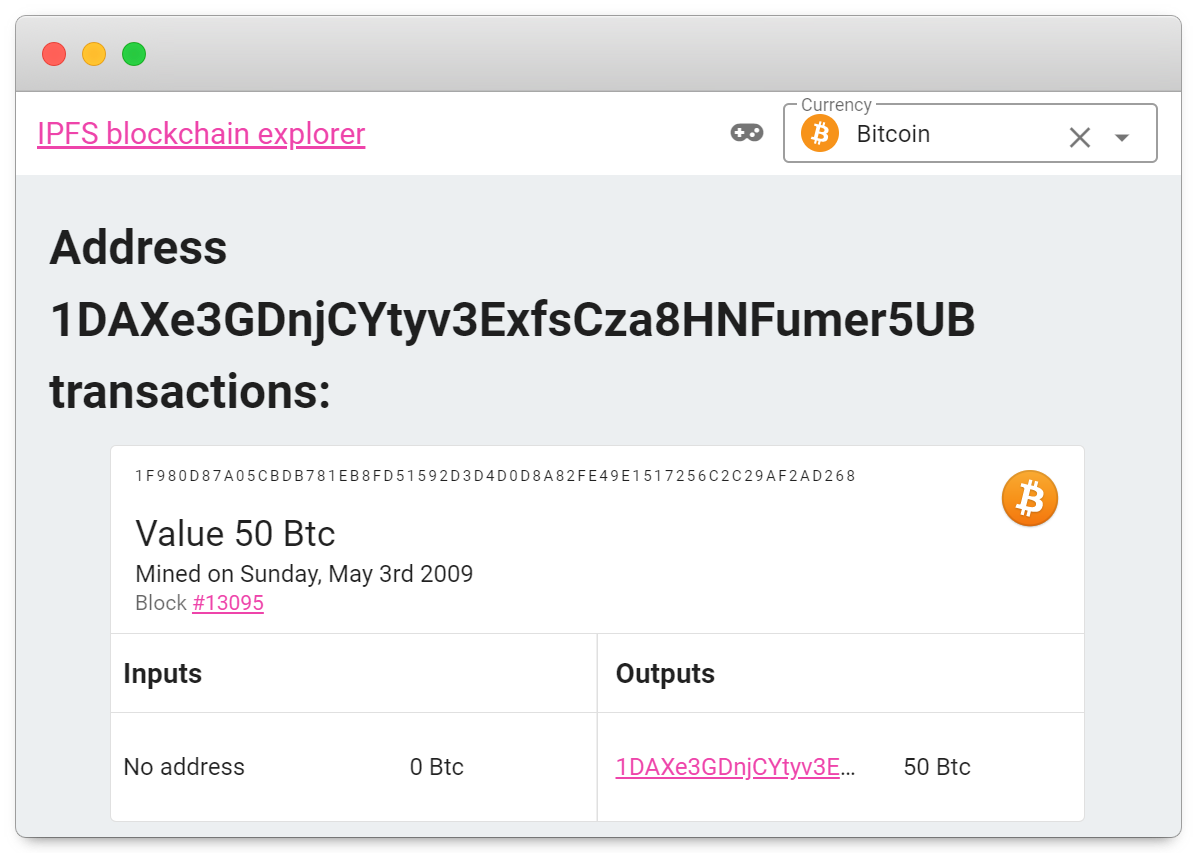
\includegraphics[width=1.0\linewidth]{explorerGuiAddressFrame.png}
        \caption{Address view}
        \label{addressView}
    \end{subfigure}%
    \begin{subfigure}[t]{.5\textwidth}
        \centering
        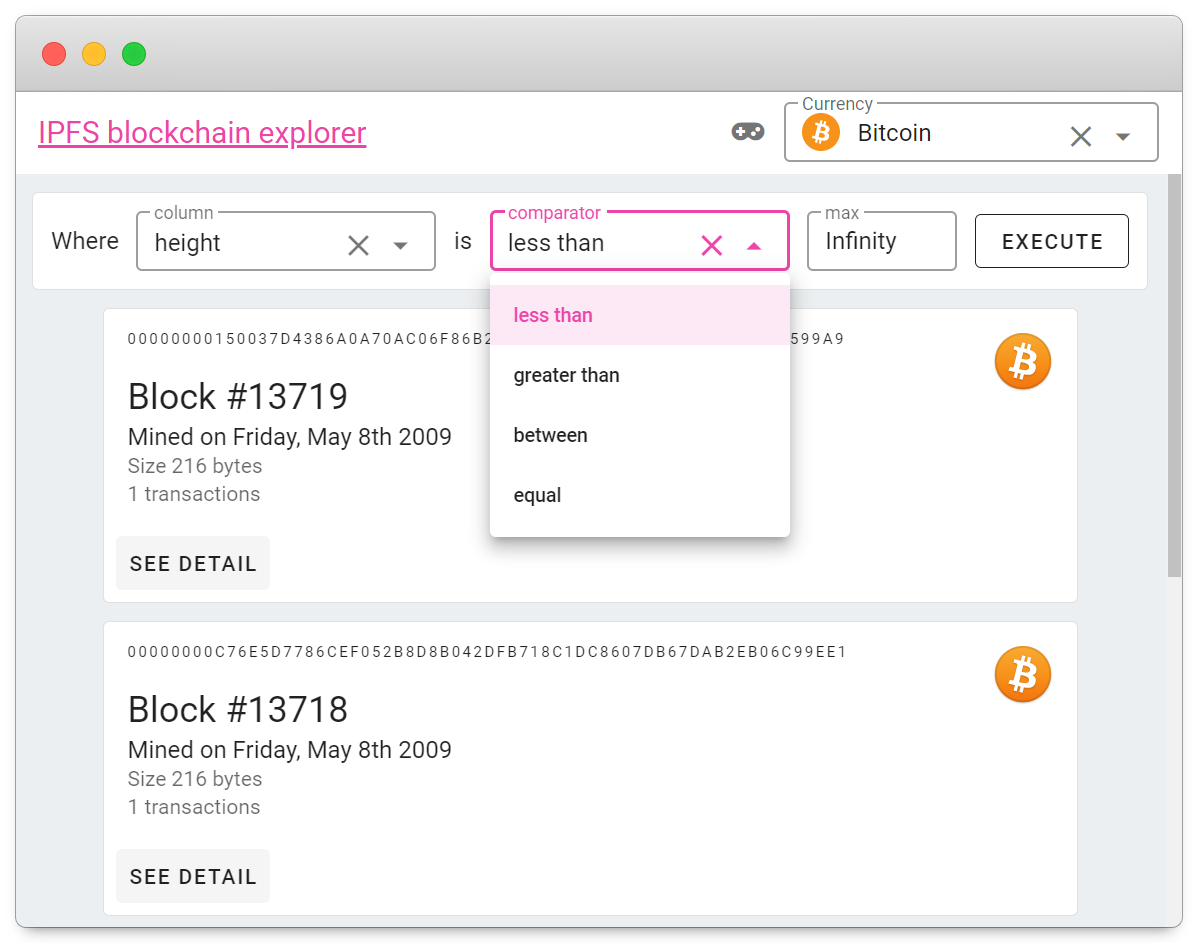
\includegraphics[width=1.0\linewidth]{explorerGuiBlocksFrame.png}
        \caption{Blocks view}
        \label{blocksView}
    \end{subfigure}
    \caption{ExplorerGUI views}
\end{figure}


After page with ExplorerGUI is loaded, it tries to connect to all supported blockchains. The home screen contains all enabled cryptocurrencies with their statuses (see Figure \ref{homeView}). Blocks list view (Figure \ref{blocksView}) is displayed when a user selects specific cryptocurrency. A~user can filter blocks by all blocks indexes in this view. A~default filter gets all blocks with height less than infinity. This query sorts blocks from the newest (highest) to the oldest (see Figure \ref{blocksView}). When a user clicks on the Execute button, ExplorerGUI starts loading blocks that match the selected query by the asynchronous algorithm shown in Figure \ref{blocksLoading}. First, we use \texttt{iterate} function (implemented in Explorer-core module) to obtain iterator over subtree of all results. This function is asynchronous, so it does not block the main JavaScript thread while it is searching the whole index and looking for the subtree. Then we create an array of promises\footnote{\url{https://developer.mozilla.org/en-US/docs/Web/JavaScript/Reference/Global_Objects/Promise}} in which the individual blocks that are displayed on the page are loaded. In for cycle, we push asynchronous tasks to the array. A~task contains single parameter that is \texttt{pagePosition}. This parameter is the order of the block that tasks loads. Every task for each block then runs in parallel. First, task calls the \texttt{next} function on subtree iterator. This function returns the next block in the subtree. The \texttt{next} function can return left or right sibling of the current block. It depends on the condition. A~subtree is traversed to the left if \texttt{greaterThan} or \texttt{between} condition is used and to the right if there is \texttt{lessThan} condition. The \texttt{next} function returns a pair of \texttt{blockPromise} which is a task that loads blockchain block from IPFS and \texttt{done} that is boolean, which signals if there are any more results in the subtree. Finally, task waits until blocks are loaded, and then assigns block in the right index of the blocks array. Thanks to this optimized asynchronous algorithm, all blocks displayed on the page are loaded in parallel.

\begin{figure}[h]
    \centering
    \begin{lstlisting}[style=ES6]
const subtree = await query.iterate()
const tasks = [];
for (let i = 0; i < pageSize; i++) {
    tasks.push(
        (async pagePosition => {
            const { blockPromise, done } = await subtree.iterator.next();
            if (done)
                return;
            blocks[page - 1 * pageSize + pagePosition] = await blockPromise;
        })(i),
    );
}
await Promise.all(tasks);
    \end{lstlisting}
    \caption{Loading blocks from database}
    \label{blocksLoading}
\end{figure}



When a user clicks on a block from the Block view, he is redirected to the Block detail view (see Figure \ref{blockDetailView}). All transactions that are confirmed in this block are listed here. Transactions have inputs and output that are usually cryptocurrency address (input can also be a coin base). Every address in a transaction in link to the Address View (see Figure \ref{addressView}). The Address view contains all transactions that address is part of as input or output.

\begin{figure}[h]
    \centering
    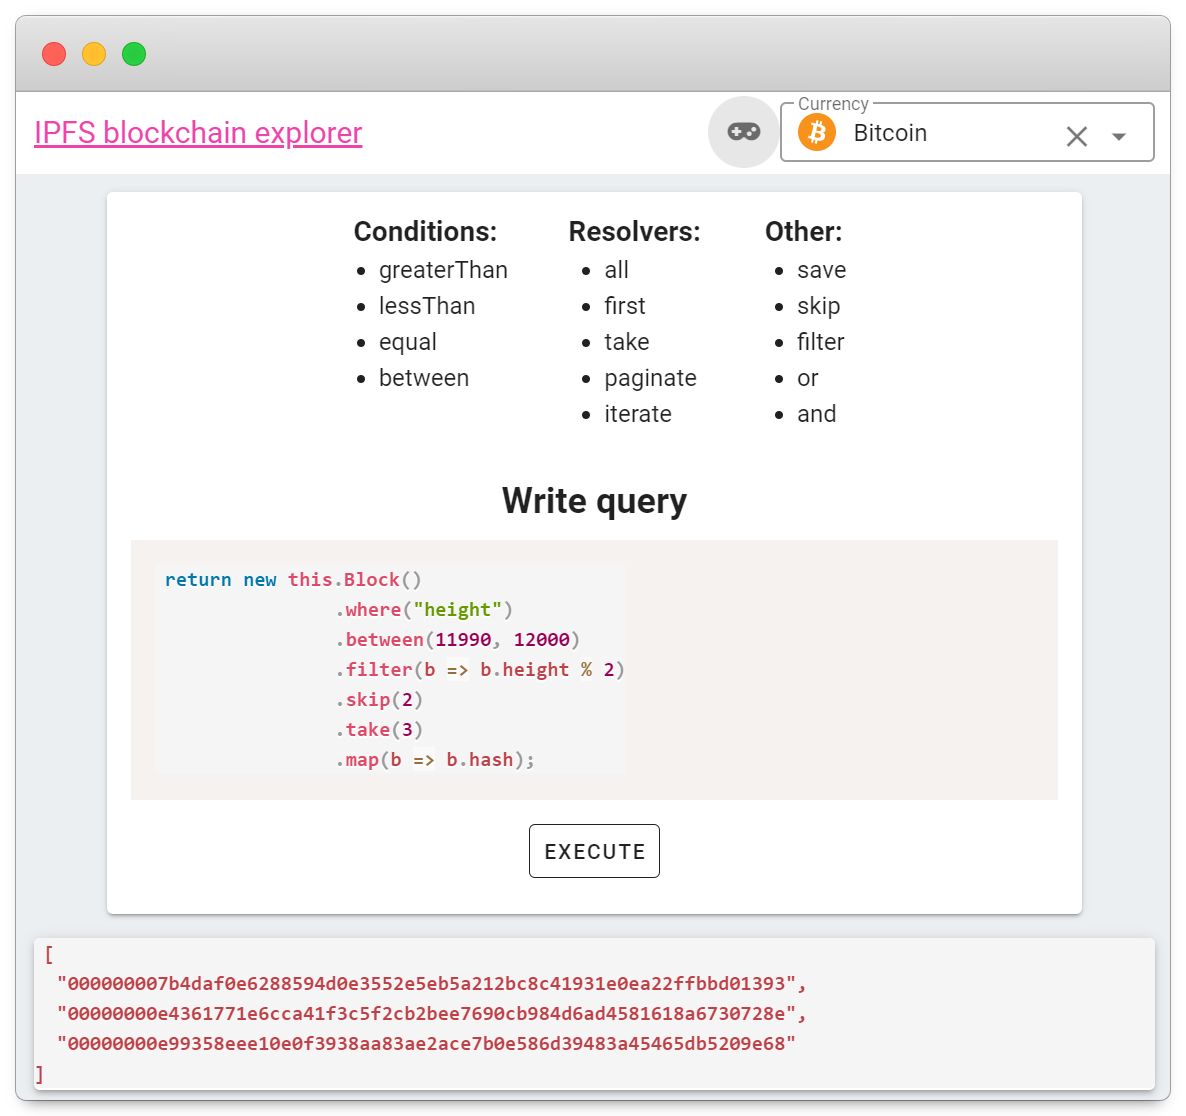
\includegraphics[width=13cm]{explorerGuiPlaygroundFrame.png}
    \caption{Playground view}
    \label{playgroundView}
\end{figure}

The last view that we implemented in ExplorerGUI is Playground (see Figure \ref{playgroundView}). In this view, the user can write a query to the web editor and execute it. Syntax highlighting in editor is done by Prism\footnote{\url{https://prismjs.com/}}. Result of a user query is returned in JSON format bellow query.


\subsection{ExplorerAPI}
ExplorerAPI is a server-side application that provides simple HTTP API.
After ExplorerAPI starts, it connects to the all enabled cryptocurrency databases (specified in \texttt{.env} file). Then it registers all three controllers (for blocks, transactions and addresses) and starts HTTP server on port described in \texttt{.env} file or \texttt{5000} if there is no specific port in the environment file. ExplorerAPI has only three endpoints (\texttt{block}, \texttt{address} and \texttt{transaction}). All these endpoints accepts query parameter (in case of \texttt{GET} method) or body parameter (\texttt{POST} method) in which query is described (see Figure \ref{explorerApiRequest}). This parameter can consist of array of conditions and filters, skip property and resolver. The parameter is translated to the Query system and result is return in JSON format (see Figure \ref{explorerApiResponse}). ExplorerAPI can accept multiple connections at once, because each request is processed in separated promise (task).


